\subsection{Misc}

\begin{center}
  \begin{tikzpicture}[bgnd/.style={circle, fill=white, draw=white}]
    %\node[opacity=0.2] at (0,0) {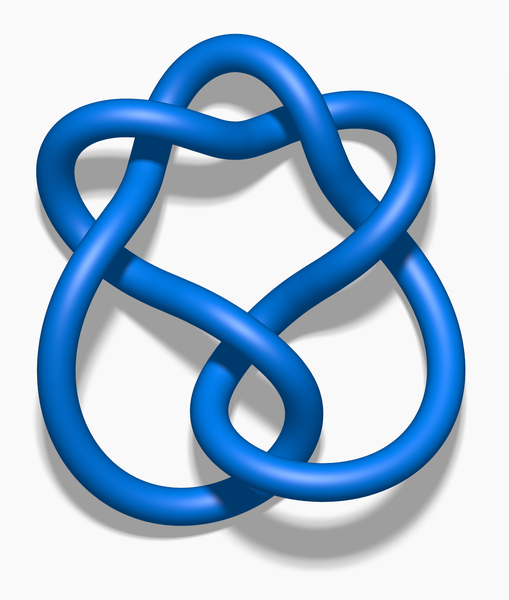
\includegraphics[width=0.7\textwidth]{./rozdzialy/6_1-3d.png}};

    \coordinate (a0) at (0,0);
    \coordinate (a1) at (90:5);
    \coordinate (a2) at (45:3);
    \coordinate (a3) at (-40:4.6);
    \coordinate (a4) at (-120:2.4);
    \coordinate (a5) at (10:0.7);
    \coordinate (a6) at (50:5);
    \coordinate (a7) at (90:3.5);
    \coordinate (a8) at (180-50:5);
    \coordinate (a9) at (170:0.7);
    \coordinate (a10) at (-70:2.4);
    \coordinate (a11) at (220:4.6);
    \coordinate (a12) at (180-45:3);

    %\foreach \i in {0,...,12} \fill (a\i) circle (2pt);

    \begin{knot}[
      clip width=20, 
      flip crossing=1,
      flip crossing=3,
      flip crossing=6
      ]
      \strand[thick, ->] (a1) to[out=0, in=90+45] (a2) to[out=-45, in=40] (a3);
      \strand[thick, ->] (a3) to[out=220, in=-90] (a4) to[out=90, in=200] (a5);
      \strand[thick, ->] (a5) to[out=20, in=-60] (a6);
      \strand[thick, ->] (a6) to[out=150, in=5] (a7);
      \strand[thick, ->] (a7) to[out=170, in=20] (a8);
      \strand[thick, ->] (a8) to[out=240, in=160] (a9);
      \strand[thick, ->] (a9) to[out=-20, in=90] (a10);
      \strand[thick, ->] (a10) to[out=-90, in=-40] (a11);
      \strand[thick, ->] (a11) to[out=140, in=180+45] (a12);
      \strand[thick, ->] (a12) to[out=45, in=180] (a1);
    \end{knot}

    \node at (80: 5) {$A$};
    \node at (-40:4) {$B$};
    \node at (45:5.5) {$C$};
    \node at (135:5.5) {$D$};
    \node at (-1.5,0.1) {$E$};
    \node at (220:4) {$F$};
    
    \node[bgnd] at (70:4.7) {$1$};
    \node[bgnd] at (25:3.9) {$2$};
    \node[bgnd] at (-90:3) {$3$};
    \node[bgnd] at (90:0.5) {$4$};
    \node[bgnd] at (110:4.7) {$5$};
    \node[bgnd] at (180-25:3.9) {$6$};

    \draw[dashed] (70: 4) circle (0.4);
    \draw[dashed] (28: 3.1) circle (0.4);
    \draw[dashed] (-90:3.5) circle (0.4);
    \draw[dashed] (-90:0.15) circle (0.4);
    \draw[dashed] (180-28:3.1) circle (0.4);
    \draw[dashed] (110:4) circle (0.4);
  \end{tikzpicture}
\end{center}
Tutaj mamy
$$f=\begin{pmatrix}
  -1 & 0 & 0 & 0 & 0 & 0 \\ 
  0 & -1 & 0 & 0 & 0 & 0 \\ 
  0 & 0 & t & 0 & 0 & 0 \\ 
  0 & 0 & 0 & t & 0 & 0 \\ 
  0 & 0 & 0 & 0 & -2x^{-2}+5x^{-1}-2 & 0 \\ 
  0 & 0 & 0 & 0 & 0 & 0 
\end{pmatrix}$$
